%& -shell-escape
\documentclass[12pt, a4paper]{article}

\usepackage[hmargin=2.5cm, vmargin=2cm]{geometry}
\usepackage{amsthm, amssymb, mathtools, yhmath, graphicx}
\usepackage{fontspec, type1cm, titlesec, titling, fancyhdr, tabularx}
\usepackage{color}
\usepackage{unicode-math}
\usepackage{float}
\usepackage{hhline}
\usepackage{comment}
\usepackage[abbreviation,per-mode=symbol]{siunitx}
\usepackage{csvsimple}
\usepackage{subcaption}
\usepackage[CheckSingle, CJKmath]{xeCJK}
\usepackage{CJKulem}
\usepackage{enumitem}
\usepackage{tikz}
\usepackage[siunitx]{circuitikz}
\usepackage{wrapfig}
%\setCJKmainfont[BoldFont=cwTex Q Hei]{cwTex Q Ming}
%\setCJKsansfont[BoldFont=cwTex Q Hei]{cwTex Q Ming}
%\setCJKmonofont[BoldFont=cwTex Q Hei]{cwTex Q Ming}
\setCJKmainfont[BoldFont=cwTeX Q Hei]{cwTeX Q Ming}

\def\normalsize{\fontsize{12}{18}\selectfont}
\def\large{\fontsize{14}{21}\selectfont}
\def\Large{\fontsize{16}{24}\selectfont}
\def\LARGE{\fontsize{18}{27}\selectfont}
\def\huge{\fontsize{20}{30}\selectfont}

%\titleformat{\section}{\bf\Large}{\arabic{section}}{24pt}{}
%\titleformat{\subsection}{\large}{\arabic{subsection}.}{12pt}{}
%\titlespacing*{\subsection}{0pt}{0pt}{1.5ex}

\parindent=24pt

\DeclarePairedDelimiter{\abs}{\lvert}{\rvert}
\DeclarePairedDelimiter{\norm}{\lVert}{\rVert}
\DeclarePairedDelimiter{\inpd}{\langle}{\rangle}
\DeclarePairedDelimiter{\ceil}{\lceil}{\rceil}
\DeclarePairedDelimiter{\floor}{\lfloor}{\rfloor}

\newcommand{\unit}[1]{\:(\text{#1})}
\newcommand{\df}[1]{\mathop{}\!\mathrm{d^#1}}
\newcommand{\img}{\mathrm{i}}
\newcommand{\dD}{\mathrm{d}}
\newcommand{\dI}{\,\mathrm{d}}
\newcommand{\paral}{\mathbin{\|}}

\title{ \bf {\Huge 電子電路實驗7:Power Amplifiers}\\ 實驗結報}
\author{B02901178 江誠敏}

\begin{document}

\maketitle


\section{實驗結果}
\subsection{改變 $V_{DC}$,量測 $V_O$}
\begin{center}
	\begin{tabular}{p{3cm}p{4.5cm}}
	\hline
  $V_{DC}$ & $V_{O}$ \\
  \hline
  \hline
  $\SI{5}\V$ & $\SI{13.448}\V$ \\
  \hline
  $\SI{10}\V$ & $\SI{13.486}\V$ \\
  \hline
  $\SI{15}\V$ & $\SI{13.527}\V$ \\
  \hline
  \end{tabular}
\end{center}

\subsection{改變 $R_1$,量測 $V_O$}
\begin{center}
	\begin{tabular}{p{3cm}p{4.5cm}}
	\hline
  $R_{1}$ & $V_{O}$ \\
  \hline
  \hline
  $\SI{1}\kohm$ & $\SI{8.586}\V$ \\
  \hline
  $\SI{2.5}\kohm$ & $\SI{13.315}\V$ \\
  \hline
  $\SI{10}\kohm$ & $\SI{13.484}\V$ \\
  \hline
  \end{tabular}
\end{center}

\subsection{改變 $R_L$,量測 $V_O$}
\begin{center}
	\begin{tabular}{p{3cm}p{4.5cm}}
	\hline
  $R_{L}$ & $V_{O}$ \\
  \hline
  \hline
  $\SI{50}\kohm$ & $\SI{13.474}\V$ \\
  \hline
  $\SI{100}\kohm$ & $\SI{13.484}\V$ \\
  \hline
  \end{tabular}
\end{center}

\section{結報問題}

\begin{enumerate}[itemsep=20pt, topsep=10pt]

  \item {\bf When designing the linear regulator, what is the relation between the 
    transistor $Q_1$ and output power? Describe the answer by words or 
 mathematical expressions.   } \\[10pt]
 答: 由講義的推導我們有 $V_o \approx (1 + R_1 / R_2) V_r$ ,最多差一個 $V_{BE} \approx
 \SI{0.7}\V$ 的誤差。 並且 $V_{BE}$ 不管 BJT 的異同都會差不多是 $\SI{0.7}\V$ , 而輸出的
 Power 為
 \[ P_o = V_o \frac{R_L}{R_L + \SI{200}\ohm} \frac{V_o}{R_L + \SI{200}\ohm} \]
 和 BJT 一點關係都沒有,所以這題我想破頭都還是覺得 $Q_1$ 跟 Output Power 一點關係都沒有…

  \item {\bf What region should the transistor $Q_1$ be operated? In active region or 
 saturation region? Please try to analyze the question with the theory or 
 measured data. } \\[10pt]
    答: The trainsistor $Q_1$ should be operated in active region. 因為如果 BJT 是在 saturation
    ,則由 $V_{CE} \approx 0.4$ 可知此時 $V_o \approx V_{DC} - \SI{0.4}\V$ ,但這不是我們想要的,
    因為 $V_{DC}$ 不見得是穩定的電壓源, 我們想要的是希望 $V_o$ ``follow"
    由 Zener Diode 的 $V_r$ 所產生的穩定電壓 $V_{B}$ , 因此我們應該讓 BJT 在 active mode 下運
    作。 此時 $V_o \approx V_{B} - \SI{0.7}\V$ 。 

  \item {\bf 請問 PNP 與 NPN BJT 的 $\beta$ 值,即 $\beta_p$ 與 $\beta_n$ 誰比較大?原因是? } \\[10pt]
    答: 我去查了一下 NPN 和規格上與其互補的 PNP 的 $\beta$ 值 (如 2N2222, 2N2907) ,發現好像差不多。
    不過應該是 NPN 的 $\beta$ 比較大 , 因為電子的 mobility 比較大 , 因此 PNP 的 $I_B$ 會比較大 (
    電子較易流到 C 端), 而 $\beta = I_C / I_B$ ,所以 $\beta$ 較小。

  \item {\bf 請說明穩壓電路的好處,並列舉三種常用的穩壓IC及其規格。 } \\[10pt]
  答: 穩壓電路的電壓比較穩定,電子元件較不會因為突然的電壓不穩定或是雜訊而失效。\\
  常見的有
  \begin{enumerate}
    \item LM317: 可條控的 Linear voltage regulator, 電壓範圍可從 $\SI{1.25}\V$ 到 $\SI{40}\V$。
    \item LM78 系列: 各種固定的 Linear voltage regulator, 電壓範圍有最低 $\SI{5}\V$ 到最高 $\SI{24}\V$。
    \item LM79 系列: 與LM78 類似,不過輸出電壓是負的。
  \end{enumerate}
\item {\bf 請描述功率晶體或高速元件的散熱機制,並列舉三種常用的散熱材料、外觀樣貌及其規格。 } \\[10pt]
  答: 基本上都是將高耗能的 IC 與散熱裝制相連, 使散熱裝制將熱傳導出去。
  常見的有

  \begin{enumerate}
    \item 散熱片: 片狀的導熱材料,通常用金屬(如鋁、銅)或是陶瓷等等材料做成。 

      \begin{minipage}[t]{\linewidth}
        \centering
        \begin{figure}[H]
        \centering
        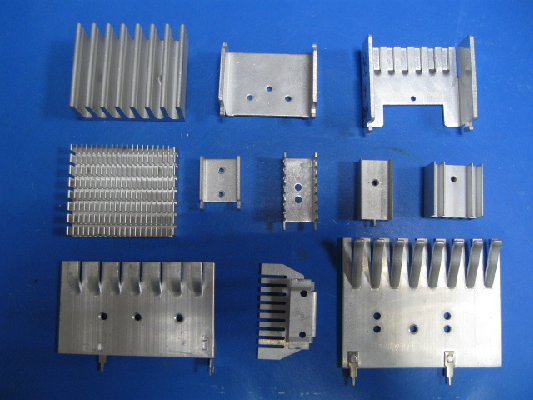
\includegraphics[width=0.5\textwidth]{p1.pdf}
        \caption{一些散熱片}
      \end{figure}
      \end{minipage}
    \item 散熱膏: 材料通常是用矽油,用來填充在組件間不完全平坦所造成的細縫。其導熱速率比空氣好,因此
      可幫助散熱。 \par
      \begin{minipage}[t]{\linewidth}
        \centering
        \begin{figure}[H]
        \centering
        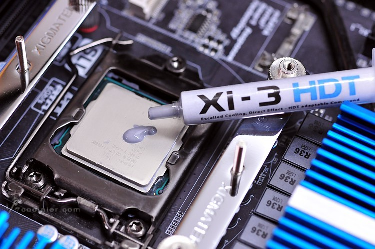
\includegraphics[width=0.5\textwidth]{p2.pdf}
        \caption{塗在 CPU 上的散熱膏}
      \end{figure}
      \end{minipage}
    \item 其他外在散熱裝置: 如風扇、水冷裝置等等… \par
      \begin{minipage}[t]{\linewidth}
        \centering
        \begin{figure}[H]
        \centering
        \begin{subfigure}{0.49\textwidth}
          \centering
          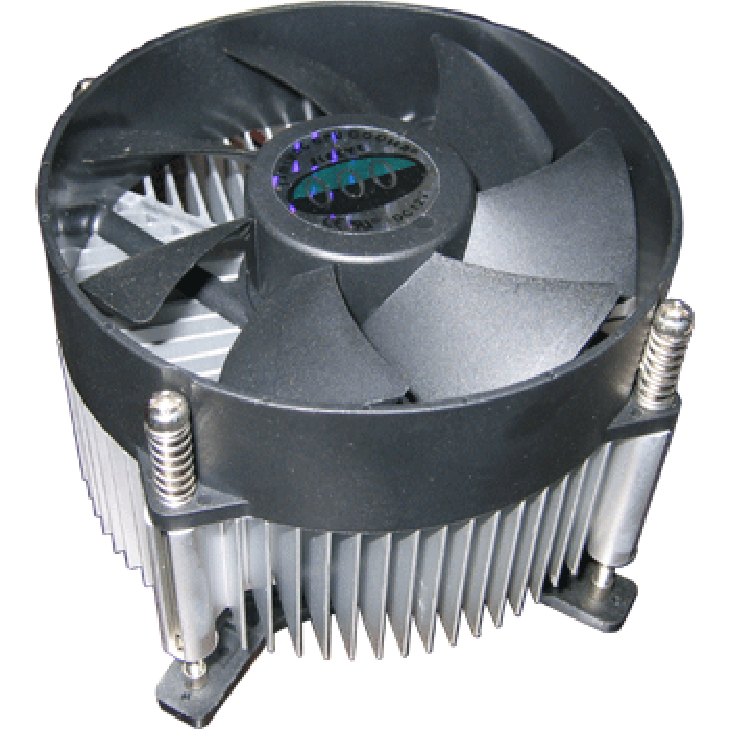
\includegraphics[width=0.5\textwidth]{p3.pdf}
          \caption{風扇冷卻裝置}
        \end{subfigure}%
        \begin{subfigure}{0.49\textwidth}
          \centering
          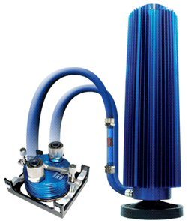
\includegraphics[width=0.5\textwidth]{p4.pdf}
          \caption{水冷卻裝置}
        \end{subfigure}
      \end{figure}
      \end{minipage}
  \end{enumerate}
\item {\bf 請描述何謂負回授? } \\[10pt]
    答: 負回授即將輸出接回輸入,並且所造成的影響和原來的變動相反。如此可以穩定系統必免
    太劇烈的變化。 \\
    如這個實驗將 $\beta V_o$ 接回原本的負輸出,使最後的輸出電壓變為
    \[ V_o = \frac{A}{1+\beta A} V_i \approx \frac{1}{\beta} V_i \]
    與原先 $V_o = A V_i$ 相比可以穩定許多。
\end{enumerate}

\section{心得}
今天是本學期最後一次做實驗! 結果最後一次的實驗好像相對比較簡單,可惜考試大概是不
會考這一題了! 希望下一次考實驗時儀器不要突然壞掉就好! 想到這裡我還是趕快拿點
乖乖去廟裡拜拜比較實際!
\end{document}

